% file: 3-9-connectivity.tex

\documentclass[]{beamer}
% File: preamble.tex
\usepackage{lmodern}

\usepackage{xeCJK}
\usetheme{CambridgeUS} % try Pittsburgh
\usecolortheme{beaver}
\usefonttheme[onlymath]{serif} % try "professionalfonts"

\setbeamertemplate{itemize items}[default]
\setbeamertemplate{enumerate items}[default]

\usepackage{comment}

\usepackage{amsmath, amsfonts, latexsym, mathtools, tabu}
\newcommand{\set}[1]{\{#1\}}
\newcommand{\ps}[1]{\mathcal{P}(#1)}
\usepackage{bm}
\DeclareMathOperator*{\argmin}{\arg\!\min}

\ExplSyntaxOn
\bool_new:N \l__xeCJK_listings_letter_bool
\ExplSyntaxOff
\usepackage{listings}

\definecolor{bgcolor}{rgb}{0.95,0.95,0.92}

\lstdefinestyle{CStyle}{
    language = C,
    basicstyle = \ttfamily\bfseries,
    backgroundcolor = \color{bgcolor},   
    keywordstyle = \color{blue},
    stringstyle = \color{teal},
    commentstyle = \color{cyan},
    breakatwhitespace = false,
    breaklines = true,                 
    mathescape = true,
    escapeinside = ||,
    morekeywords = {procedure, end, foreach, repeat, until},
    showspaces = false,                
    showstringspaces = false,
    showtabs = false,                  
}

% colors
\newcommand{\red}[1]{\textcolor{red}{#1}}
\newcommand{\redoverlay}[2]{\textcolor<#2>{red}{#1}}
\newcommand{\green}[1]{\textcolor{green}{#1}}
\newcommand{\greenoverlay}[2]{\textcolor<#2>{green}{#1}}
\newcommand{\blue}[1]{\textcolor{blue}{#1}}
\newcommand{\blueoverlay}[2]{\textcolor<#2>{blue}{#1}}
\newcommand{\purple}[1]{\textcolor{purple}{#1}}
\newcommand{\cyan}[1]{\textcolor{cyan}{#1}}
\newcommand{\teal}[1]{\textcolor{teal}{#1}}

% colorded box
\newcommand{\rbox}[1]{\red{\boxed{#1}}}
\newcommand{\gbox}[1]{\green{\boxed{#1}}}
\newcommand{\bbox}[1]{\blue{\boxed{#1}}}
\newcommand{\pbox}[1]{\purple{\boxed{#1}}}

\usepackage{pifont}
\usepackage{wasysym}

\newcommand{\cmark}{\green{\ding{51}}}
\newcommand{\xmark}{\red{\ding{55}}}
%%%%%%%%%%%%%%%%%%%%%%%%%%%%%%%%%%%%%%%%%%%%%%%%%%%%%%%%%%%%%%
% for fig without caption: #1: width/size; #2: fig file
\newcommand{\fignocaption}[2]{
  \begin{figure}[htp]
    \centering
      \includegraphics[#1]{#2}
  \end{figure}
}

\usepackage{tikz}
\usetikzlibrary{positioning, mindmap, shadows}

\newcommand{\push}{\texttt{Push}}
\newcommand{\pop}{\texttt{Pop}}

\newcommand{\titletext}{2-3 Counting}

\newcommand{\thankyou}{
  \begin{frame}[noframenumbering]{}
    \fignocaption{width = 0.50\textwidth}{figs/thankyou.png}
  \end{frame}
}

%%%%%%%%%%%%%%%%%%%%
\title[\titletext]{\titletext}
% \subtitle{}

\author[Hengfeng Wei]{Hengfeng Wei}
\titlegraphic{
\includegraphics[height = 2.0cm]{figs/qrcode-problem-solving-2018-autumn}}
\institute{hfwei@nju.edu.cn}
\date{November $26$, $2018$}

\AtBeginSection[]{
  \begin{frame}[noframenumbering, plain]
    \frametitle{\titletext}
    \tableofcontents[currentsection, sectionstyle=show/shaded, subsectionstyle=show/show/hide]
  \end{frame}
}
%%%%%%%%%%
\begin{document}
\maketitle

% file: overview.tex

%%%%%%%%%%%%%%%
\begin{frame}{}
  \begin{columns}
    \column{0.50\textwidth}
      \fignocaption{width = 0.55\textwidth}{figs/chai}
    \column{0.50\textwidth}
      \pause
      \fignocaption{width = 0.85\textwidth}{figs/xiongan}
  \end{columns}

  \pause
  \vspace{0.50cm}
  \begin{center}
    {\red{\large $Q:$ What is Probability?}} \\[5pt] \pause
    {\violet{\small (Objective? \quad Subjective? \quad Neutral?)}}
  \end{center}
\end{frame}
%%%%%%%%%%%%%%%

%%%%%%%%%%%%%%%
\begin{frame}{}
  \begin{columns}
    \column{0.35\textwidth}
      \fignocaption{width = 0.95\textwidth}{figs/infinity}
    \column{0.30\textwidth}
      \fignocaption{width = 0.70\textwidth}{figs/intuition-told}
    \column{0.35\textwidth}
      \fignocaption{width = 0.90\textwidth}{figs/dice}
  \end{columns}

  \vspace{0.50cm}
  \begin{quote}
    ``\ldots and the many \purple{paradoxes} show clearly that we, as humans, 
    \purple{lack a well grounded intuition} in this matter.''

    \hfill --- {\small ``The Art of Probability'', Richard W. Hamming}
  \end{quote}

  \pause
  \begin{quote}
    ``When called upon to judge probability, people actually judge something else
    and \purple{\bf believe} they have judged probability.''

    \hfill --- {\small ``Thinking, Fast and Slow'', Daniel Kahneman}
  \end{quote}
\end{frame}
%%%%%%%%%%%%%%%

%%%%%%%%%%%%%%%
\begin{frame}{}
  \fignocaption{width = 0.30\textwidth}{figs/Leibniz}

  \pause
  \vspace{0.50cm}
  \begin{quote}
    \centerline{\red{\LARGE Let us calculate [calculemus].}}
  \end{quote}
\end{frame}
%%%%%%%%%%%%%%%

%%%%%%%%%%%%%%%
\begin{frame}{}
  \fignocaption{width = 0.30\textwidth}{figs/open-topics}

  {\large
    \begin{enumerate}[(a)]
      \centering
      \setlength{\itemsep}{6pt}
      \item Monty Hall problem
      \item Boy or Girl paradox
      \item Searching unsorted array
    \end{enumerate}
  }
\end{frame}
%%%%%%%%%%%%%%%

%%%%%%%%%%%%%%%
% \begin{frame}{}
%   \fignocaption{width = 0.45\textwidth}{figs/intuition-vs-calculation}
% 
%   \vspace{0.50cm}
%   \begin{quote}
%     \centerline{\red{\LARGE Intuition {\it vs.} Calculation}}
%   \end{quote}
% \end{frame}
%%%%%%%%%%%%%%%

% file: sections/2conn.tex

%%%%%%%%%%%%%%%%%%%%
\begin{frame}{}
  \begin{exampleblock}{2-Connectivity (Problem $5.10$)}
    \begin{center}
      A connected graph $G$ with $m \ge 2$ is \red{\it nonseparable} \\[3pt]
      $\iff$ \\[3pt]
      any two \red{\it adjacent} edges of $G$ lie on a common cycle of $G$.
    \end{center}
  \end{exampleblock}

  \pause
  \begin{proof}
    \begin{center}
      ``$\implies$''
    \end{center}

    \pause
    \vspace{-0.30cm}
    \begin{columns}
      \column{0.65\textwidth}
	\begin{align*}
	  &G \text{ is nonseparable} \\
	  &\implies u, w \text{ lie on a common cycle} \\
	  \uncover<4->{
	    &\implies \exists \text{ path } u \sim w \uncover<6->{\red{\text{ that does not contain $v$}}} \\
	    &\implies \exists \text{ cycle } u - v - w \sim u
	  }
	\end{align*}
      \column{0.30\textwidth}
	% file: 3-9-connectivity/2conn-adjacent-edges.tex

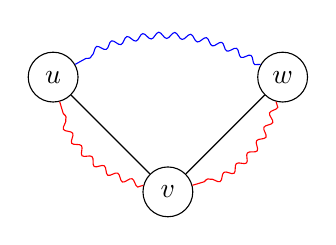
\begin{tikzpicture}[every node/.style = {draw, circle, minimum size = 18pt},
    path/.style = {-, decorate, decoration = {snake, amplitude = .4mm, segment length = 2mm, post length = 1mm}}]
  \node (v) {$v$};
  \node (u) [above left = of v] {$u$};
  \node (w) [above right = of v] {$w$};

  \path (v) edge (u)
  	    edge (w);

  \uncover<4->{
    \path (w) edge[blue, bend right, path] (u);
  }

  \uncover<5->{
    \path (w) edge[red, bend left, path] (v)
	  (v) edge[red, bend left, path] (u);
  }
\end{tikzpicture}
    \end{columns}
  \end{proof}
\end{frame}
%%%%%%%%%%%%%%%%%%%%

%%%%%%%%%%%%%%%%%%%%
\begin{frame}{}
  \begin{exampleblock}{2-Connectivity (Problem $5.10$)}
    \begin{center}
      A connected graph $G$ with $m \ge 2$ is \red{\it nonseparable} \\[3pt]
      $\iff$ \\[3pt]
      any two \red{\it adjacent} edges of $G$ lie on a common cycle of $G$.
    \end{center}
  \end{exampleblock}

  \begin{proof}
    \begin{center}
      ``$\Longleftarrow$'' \\[6pt]
      \purple{By Contradiction.}
    \end{center}

    \pause
    \vspace{-0.30cm}
    \begin{columns}
      \column{0.65\textwidth}
	\begin{align*}
	  &\text{Suppose } v \text{ is a cut-vertex of } G \\
	  &\implies G - v \text{ contains} \ge 2 \text{ comps } G_1, G_2, \cdots \\
	  &\implies \exists u \in G_1, w \in G_2: v-u \land v-w \\
	  &\implies v-u, v-w \text{ lie on a common cycle} \\
	  &\implies \exists \text{ path } u \sim w \text{ that does not contain } v \\
	\end{align*}
      \column{0.35\textwidth}
	\fig{width = 0.70\textwidth}{figs/2conn-cut-vertex}
    \end{columns}
  \end{proof}
\end{frame}
%%%%%%%%%%%%%%%%%%%%

%%%%%%%%%%%%%%%%%%%%
\begin{frame}{}
  \begin{columns}
    \column{0.50\textwidth}
      \fig{width = 0.70\textwidth}{figs/cut-vertex-structure}

      \[
	\forall G_i\; \exists v_i \in G_i\; v - v_i
      \]
    \column{0.50\textwidth}
      \pause
      \fig{width = 0.70\textwidth}{figs/2conn-cut-vertex}

      \pause
      \[
	\red{\forall v \in S}\; \forall G_i\; \exists v_i \in G_i\; v - v_i
      \]
  \end{columns}
\end{frame}
%%%%%%%%%%%%%%%%%%%%

%%%%%%%%%%%%%%%%%%%%
\begin{frame}{}
  \begin{exampleblock}{2-Connectivity (Problem $5.10$)}
    \begin{center}
      A connected graph $G$ with $m \ge 2$ is \red{\it nonseparable} \\[3pt]
      $\iff$ \\[3pt]
      any two \red{\it adjacent} edges of $G$ lie on a common cycle of $G$.
    \end{center}
  \end{exampleblock}

  \pause
  \vspace{0.60cm}
  \begin{exampleblock}{2-Connectivity (Extended Problem)}
    \begin{center}
      A connected graph $G$ with $m \ge 2$ is \red{\it nonseparable} \\[3pt]
      $\iff$ \\[3pt]
      \red{any two edges} of $G$ lie on a common cycle of $G$.
    \end{center}
  \end{exampleblock}
\end{frame}
%%%%%%%%%%%%%%%%%%%%

% file: sections/kconn.tex

%%%%%%%%%%%%%%%%%%%%
\begin{frame}{}
  \begin{exampleblock}{Expansion Lemma (Problem $5.34$; Theorem $5.18$)}
    Let $G$ be a $k$-connected graph and let $S$ be any set of $k$ vertices. \\[8pt]
    If a graph $H$ is obtained from $G$ by \red{adding a new vertex $w$ and joining $w$ to the vertices of $S$},
    then $H$ is also $k$-connected.
  \end{exampleblock}

  \vspace{0.80cm}
  \fig{width = 0.40\textwidth}{figs/expansion-lemma}
\end{frame}
%%%%%%%%%%%%%%%%%%%%

%%%%%%%%%%%%%%%%%%%%
\begin{frame}{}
  \begin{columns}
    \column{0.40\textwidth}
      \fig{width = 0.80\textwidth}{figs/expansion-lemma}
    \column{0.60\textwidth}
      \[
	\text{To prove } \kappa(H) \ge k
      \]

      \pause
      \begin{center}
	Let $U$ be a vertex-cut of $H$. \\[5pt]
	\red{We prove that $|U| \ge k$.}
      \end{center}
  \end{columns}

  \pause
  \vspace{0.50cm}
  \begin{columns}[t]
    \column{0.50\textwidth}
      \begin{center}
	\purple{\textsc{Case I:} $U$ is a vertex-cut of $G$}
      \end{center}

      \uncover<4->{
	\[
	  |U| \ge k
	\]
      }
    \column{0.50\textwidth}
      \begin{center}
	\purple{\textsc{Case II:} $U$ is not a vertex-cut of $G$}
      \end{center}

      \vspace{-0.60cm}
      \begin{gather*}
	\uncover<5->{ w \in U } \\[3pt]
	\uncover<6->{ U - w \text{ is a vertex-cut of } G } \\[3pt]
	\uncover<7->{ |U| \ge k + 1 }
      \end{gather*}
  \end{columns}
\end{frame}
%%%%%%%%%%%%%%%%%%%%

%%%%%%%%%%%%%%%%%%%%
\begin{frame}{}
  \begin{exampleblock}{2-Connectivity (Extended Problem)}
    \begin{center}
      A connected graph $G$ with $m \ge 2$ is \red{\it nonseparable} \\[3pt]
      $\iff$ \\[3pt]
      \red{any two edges} of $G$ lie on a common cycle of $G$.
    \end{center}
  \end{exampleblock}

  \pause
  \[
    \implies
  \]
  \begin{center}
    Consider two edges $uv$ and $xy$.
  \end{center}

  \pause
  \begin{columns}
    \column{0.50\textwidth}
      \uncover<4->{
	\begin{center}
	  Add $w, z$ \\[5pt]
	  Add $wu, wv; zx, zy$ \\[5pt]
	  $w$ and $z$ lie on a common cycle
	\end{center}
      }
    \column{0.50\textwidth}
      \fig{width = 0.60\textwidth}{figs/2conn-edges-cycle}
  \end{columns}
\end{frame}
%%%%%%%%%%%%%%%%%%%%

% file: sections/remove-edge.tex

%%%%%%%%%%%%%%%%%%%%
\begin{frame}{}
  \begin{exampleblock}{Effects of Removing an Edge on Connectivity (Problem $5.22$\; (a))}
    \begin{enumerate}[(a)]
      \item If $G$ is $k$-connected and $e = uv \in E(G)$, then $G - e$ is $(k-1)$-connected.
    \end{enumerate}
  \end{exampleblock}

  \pause
  \[
    \text{To prove } \kappa(G) \ge k \implies \kappa(G - e) \ge k-1
  \]

  \pause
  \vspace{0.50cm}
  \begin{center}
    Choose any $U \subseteq V(G)$ with $|U| < k - 1$. \\[6pt]
    \red{We prove that $G - e - U$ is connected.}
  \end{center}
\end{frame}
% \red{We prove that $\kappa(G - e) < \kappa(G) \implies \kappa(G - e) \ge k - 1$}
%%%%%%%%%%%%%%%%%%%%

%%%%%%%%%%%%%%%%%%%%
\begin{frame}{}
  \begin{center}
    Choose any $U \subseteq V(G)$ with $|U| < k - 1$. \\[6pt]
    \red{We prove that $G - e - U$ is connected.}
  \end{center}

  \pause
  \[
    G \text{ is } k\text{-connected} \implies G - U \text{ is connected}
  \]

  \pause
  \begin{center}
    \teal{Suppose, by contradiction, that $G - e - U$ is not connected.} \\[8pt] \pause
    $e = uv$ is a bridge of $G - U$ \\[8pt] \pause
    \textcolor<8>{red}{$U \cup \set{u}$ is a vertex-cut of $G$} \pause
    \[
      \text{But } \Big\lvert U \cup \set{u} \Big \rvert < k
    \]
  \end{center}

  \only<7->{
    \vspace{-0.50cm}
    \fig{width = 0.30\textwidth}{figs/wrong}
  }
\end{frame}
%%%%%%%%%%%%%%%%%%%%

%%%%%%%%%%%%%%%%%%%%
\begin{frame}{}
  \fig{width = 0.30\textwidth}{figs/bridge}

  \begin{columns}
    \column{0.50\textwidth}
      \pause
      \[
	\textsc{Case I}: |X| \ge 2 \lor |Y| \ge 2
      \]

      \pause
      \begin{center}
	\red{$U \cup \set{u}$ is a vertex-cut of $G$}
      \end{center}
      \[
	\text{But } \Big\lvert U \cup \set{u} \Big \rvert < k
      \]
    \column{0.50\textwidth}
      \pause
      \[
	\textsc{Case II}: |X| = |Y| = 1
      \]

      \pause
      \vspace{-0.60cm}
      \begin{gather*}
	\onslide<5->{|U| = n - 2 < k - 1} \\[6pt]
	\onslide<6->{\red{\kappa(G) \ge k > n - 1}} \\[6pt]
	\onslide<7->{\text{But } 0 \le \kappa(G) \le n - 1}
      \end{gather*}
  \end{columns}
\end{frame}
%%%%%%%%%%%%%%%%%%%%

%%%%%%%%%%%%%%%%%%%%
\begin{frame}{}
  \begin{exampleblock}{Effects of Removing an Edge on Connectivity (Problem $5.22$\; (b))}
    \begin{enumerate}[(a)]
      \setcounter{enumi}{1}
      \item If $G$ is $k$-edge-connected and $e = uv \in E(G)$, then $G - e$ is $(k-1)$-edge-connected.
    \end{enumerate}
  \end{exampleblock}

  \[
    \lambda(G) \ge k \implies \lambda(G - e) \ge k-1
  \]

  \pause
  \vspace{0.50cm}
  \begin{center}
    Choose any $X \subseteq E(G)$ with $|X| < k - 1$. \\[6pt]
    \red{We prove that $G - e - X$ is connected.}
  \end{center}

  \pause
  \[
    G - e - X = G - (e + E) \text{ is connected} \only<4->{\;\teal{(\because \lambda(G) \ge k)}}
  \]
\end{frame}
%%%%%%%%%%%%%%%%%%%%

%%%%%%%%%%%%%%%%%%%%
\begin{frame}{}
  \[
    \kappa(G - e) \le \kappa(G)
  \]

  \pause
  \vspace{0.50cm}
  \begin{exampleblock}{Effects of Removing a Vertex on Connectivity (Extended Problem)}
    \[
      \text{Is } \kappa(G - \red{v}) \le \kappa(G)?
    \]
    \[
      \text{Is } \lambda(G - \red{v}) \le \lambda(G)?
    \]
  \end{exampleblock}

  \vspace{0.30cm}
  \only<3>{\fig{width = 0.30\textwidth}{figs/k4-k1}}

  \uncover<4->{
    \begin{exampleblock}{Effects of Removing a Vertex on Connectivity (After-class Exercise)}
      \[
	\text{Is } \kappa(G) \ge k \implies \kappa(G - v) \ge k-1?
      \]
      \[
	\text{Is } \lambda(G) \ge k \implies \lambda(G - v) \ge k-1?
      \]
    \end{exampleblock}
  }
\end{frame}
%%%%%%%%%%%%%%%%%%%%

% file/sections/lambda-delta-eq.tex

%%%%%%%%%%%%%%%%%%%%
\begin{frame}
  \begin{exampleblock}{Degree Condition for $\lambda(G) = \delta(G)$ (Problem $5.26$)}
    If $G$ is graph of order $n$ such that $\delta(G) \ge (n-1)/2$, then $\lambda(G) = \delta(G)$.
  \end{exampleblock}

  \pause
  \[
    \lambda(G) \le \delta(G)
  \]

  \begin{center}
    \red{We prove that $\lambda(G) \ge \delta(G)$.}
  \end{center}

  \pause
  \begin{columns}
    \column{0.40\textwidth}
      \fig{width = 0.60\textwidth}{figs/edge-cut-structure}
    \column{0.60\textwidth}
      \[
	\lambda(G) = |X|
      \]

      \pause
      \vspace{-0.50cm}
      \[
	1 \le |S| = k \;\red{\le n/2}, \quad |V - S| = n - k
      \]

      \pause
      \vspace{-0.50cm}
      \[
	\lambda \ge k \Big(\delta - (k - 1) \Big) \pause \ge \delta
      \]
  \end{columns}
\end{frame}
% \lambda &\ge \min \Big\{ k\big(\delta-(k-1)\big), \\ &\qquad\qquad (n-k) \big(\delta - (n-k-1) \big) \Big\} 
%%%%%%%%%%%%%%%%%%%%

%%%%%%%%%%%%%%%%%%%%
\begin{frame}
  \fig{width = 0.85\textwidth}{figs/connectivity-algs-table}
\end{frame}
%%%%%%%%%%%%%%%%%%%%

% file: sections/menger-theorem.tex



\thankyou{}
%%%%%%%%%%%%%%%
\begin{frame}[noframenumbering]
  \centerline{\large \blue{为了更好地教学, 希望能得到你的反馈、批评、意见或建议。}}

  \fignocaption{width = 0.50\textwidth}{figs/matters.png}

  \begin{center}
	{\large
	  Office 302 \\[5pt]
	  Mailbox: H016 (计算机系楼二楼) \\[5pt]
	  hfwei@nju.edu.cn }
  \end{center}
\end{frame}
%%%%%%%%%%%%%%%


\end{document}
%%%%%%%%%% 